% ------------------------------------------------------------------
\renewcommand{\thisweek}{MATH327 Week 2}
\renewcommand{\moddate}{Last modified 7 Feb.~2021}
\setcounter{section}{2}
\setcounter{subsection}{0}
\phantomsection
\addcontentsline{toc}{section}{Week 2: Micro-canonical ensemble}
\section*{Week 2: Micro-canonical ensemble}

\subsection{Statistical ensembles and thermodynamic equilibrium}
We begin this week by developing the concept of \textit{statistical ensembles} (introduced by \href{https://en.wikipedia.org/wiki/Josiah_Willard_Gibbs}{J.\ Willard Gibbs} in the early 1900s), building on the probability foundations we laid last week.
As forecast last week, we will be interested in `experiments' that simply allow a collection of degrees of freedom to evolve in time, subject to certain constraints.
At a given time $t_1$, the disposition of these degrees of freedom defines the state $\om_1$ of the system.
To consider a couple of examples, what would be a representative state for a system of $8$ \textit{spins} (arrows that can point either `up' or `down') arranged in a line?\footnote{We will consider \href{https://en.wikipedia.org/wiki/Spin_model}{spin systems} extensively in this module.  In addition to obeying simple mathematics analogous to flipping coins, spins also serve as good models of physical systems such as magnetic molecules.}
What information would characterize the state of $N$ hydrogen (H$_2$) molecules in a container?
\begin{mdframed}
  \ \\[100 pt]
\end{mdframed}

At a different time $t_2$, the system's state $\om_2$ is generally different from $\om_1$.
However, there are some measurements we can perform on these states that always produce the same outcome as the system evolves in time.
These measurements define \textit{conserved quantities}, an important example of which is the total energy $E$ \textit{inside} an isolated (or `closed') system,
\begin{equation*}
  E(\om_1) = E(\om_2).
\end{equation*}
The conservation of energy is presumably a familiar concept, and you may also know that it can be rigorously proven through \href{https://en.wikipedia.org/wiki/Emmy_Noether}{Emmy Noether}'s theorem.\footnote{This proof holds only in `flat' space-time as opposed to the curved space-time manifolds than arise in general relativity---which is far beyond the scope of this module.}
Because statistical physics was first developed when conservation of energy was primarily an empirical observation rather than a proven result, it was given a more grandiose name: the \textbf{first law of thermodynamics}.
Another way of stating the first law is that any change in the internal energy of one particular system \Om must be matched by an equal and opposite change in the energy of some other system(s) with which \Om is in contact.
We will return to this formulation of the first law in future weeks.

For now, let's return to the \textbf{examples} above, and suppose that the spin system is placed in an external magnetic field.
If a spin is parallel to the field, it contributes energy $-H$ to the total energy $E$ of the system.
If a spin is anti-parallel to the field, it instead contributes energy $H \geq 0$.
What is the total energy $E$ of a system of $N$ spins in a state with $n_+$ spins anti-parallel to the field and $n_- = N - n_+$ parallel to it?
What is $E$ for the representative $N = 8$-spin state you wrote down above?
How many of the $2^8 = 256$ states of the spin system have this energy?
\begin{mdframed}
  \ \\[100 pt]
\end{mdframed}
For the $N$ hydrogen molecules in a container, we can write a simple expression for the energy $E$ by treating each molecule as a \textit{point-like particle}, with no size or structure.
In this case each molecule contributes only its kinetic energy to $E$,
\begin{equation*}
  E = \frac{m}{2} \sum_{i = 1}^N \vec{v}_i^{\,2} = \frac{1}{2m} \sum_{i = 1}^N \vec{p}_i^{\,2},
\end{equation*}
where $\vec v_i$ is the velocity of the $i$th molecule, $\vec p_i = m \vec v_i$ is its momentum, and all molecules have exactly the same mass $m$.

As emphasized in last week's introduction, we treat the time evolution of the system as a stochastic process in which the system probabilistically adopts a sequence of states $\om_i \in \Om$:
\begin{equation*}
  \om_1 \lra \om_2 \lra \om_3 \lra \om_4 \lra \cdots
\end{equation*}
This attitude is adopted as a matter of practicality rather than one of principle.
In principle, Newton's laws would allow us to exactly predict the time evolution of (say) $\sim$$10^{23}$ hydrogen molecules, but only by specifying $\sim$$10^{23}$ initial conditions and solving $\sim$$10^{23}$ differential equations.
Since we cannot hope to write down so much information or carry out so many computations, we instead apply probability theory in order to analyze these systems.

\begin{shaded}
  This leads us to the following core definition: A \textbf{statistical ensemble} is the set of all states $\Om = \left\{\om_1, \om_2, \cdots\right\}$ that a system can possibly adopt through its time evolution.
  Each state $\om_i$ has some probability $p_i$ of being adopted by the system, so we can recognize a statistical ensemble as a probability space.
\end{shaded}

Because these states $\om_i$ depend on the `microscopic' degrees of freedom that compose the overall system, we will refer to them as \textbf{micro-states} from now on.
From last week's definition of probability, we have the requirement $\sum_i p_i = 1$, which simply means that the system must be in \textit{some} micro-state at any point in time.
The fact that time evolution cannot change any conserved quantities, as discussed above, means that such conserved quantities characterize statistical ensembles.
We will define different types of statistical ensemble that depend on the specific set of conserved quantities.

\begin{shaded}
  This week we define a \textbf{micro-canonical ensemble} to be a statistical ensemble characterized by conserved internal energy $E$ and conserved number of degrees of freedom $N$ (which we will call \textbf{particle number} for short).
\end{shaded}

According to the discussion above, this means that a system governed by the micro-canonical ensemble is \textit{isolated} in the sense that it cannot exchange energy or particles with any other system.

Now that the micro-canonical ensemble is defined, we can connect it to our intuition from everyday physical systems.
Let's consider a collection of particles moving around and bouncing (or `\textit{scattering}') off each other in a sealed container.
To a first approximation, this should describe the behaviour of air in a room, which our lived experience indicates is spread quite uniformly throughout the room in a way that is stable as time passes.
We do not expect all the air in a room to be concentrated in any one corner, nor do we expect strong collective gusts of wind without some clear external influence.

These qualitative expectations illustrate the idea of \textbf{thermodynamic equilibrium}, an axiomatic concept in statistical physics.\footnote{Our expectation that physical systems generically evolve towards thermodynamic equilibrium as time passes is more formally expressed as the \href{https://en.wikipedia.org/wiki/Ergodic_hypothesis}{ergodic hypothesis}.}
We can mathematically define thermodynamic equilibrium through the probabilities $p_i$ that appear in the micro-canonical ensemble.

\begin{shaded}
  A micro-canonical system \Om with $M$ micro-states $\om_i$ is in thermodynamic equilibrium if and only if all probabilities $p_i$ are equal.
  If $M$ is finite, the requirement $\sum_i p_i = 1$ implies
  \begin{equation}
    \label{eq:micro_equil}
    p_i = \frac{1}{M}.
  \end{equation}
\end{shaded}

The full meaning and significance of this definition are not immediately obvious, and we will continue exploring them through consideration of derived quantities such as entropy and temperature.
First, we emphasize that this equilibrium is indeed \textit{dynamic}: There is not a single `equilibrium state' that the system approaches; instead, the system continues probabilistically adopting different states as it evolves in time.
% ------------------------------------------------------------------



% ------------------------------------------------------------------
\subsection{Entropy and its properties}
\subsubsection{Definition of entropy}
We can gain further insight into thermodynamic equilibrium by considering a famous derived quantity.
\begin{shaded}
  The \textbf{entropy} of a statistical ensemble \Om with a countable number of micro-states $M$ is defined to be
  \begin{equation}
    \label{eq:entropy}
    S = - \sum_{i = 1}^M p_i \log p_i,
  \end{equation}
  where $p_i$ is the probability for micro-state $\om_i$ to occur.
  Unless otherwise specified, ``$\log$'' indicates the natural logarithm of base $e$.
\end{shaded}

When the system under consideration is in thermodynamic equilibrium, we expect derived quantities such as the entropy to be stable over time, even as different micro-states are probabilistically adopted.
This implies that such derived quantities are functions of the conserved quantities that are the same for all micro-states.
Therefore, for the micro-canonical ensemble, the equilibrium entropy $S(E, N)$ would be a function of the conserved energy and particle number.

By inserting \eq{eq:micro_equil} into \eq{eq:entropy} you can quickly compute a simple expression for the entropy of a micro-canonical ensemble in thermodynamic equilibrium:
\begin{mdframed}
  \ \\[50 pt]
\end{mdframed}
%\begin{equation}
%  \label{eq:}
%  S = - \sum_{i = 1}^M \frac{1}{M} \log \left(\frac{1}{M}\right) = \log M.
%\end{equation}
Your result should depend only on the number of micro-states $M$, and diverge as $M \to \infty$.
While the energy $E$ and particle number $N$ are not explicit in this expression, $\left\{E, N, M\right\}$ are inter-related and might be expressed in terms of each other depending on the particular situation under consideration.
For example, what is the equilibrium entropy of the system of $N$ spins considered above, if the external magnetic field is turned off (so $H = 0$ implying $E = 0$)?
\begin{mdframed}
  \ \\[100 pt]
\end{mdframed}
% ------------------------------------------------------------------



% ------------------------------------------------------------------
\subsubsection{Extensivity}
The increase in entropy for an increasing number of micro-states $M$ is a reflection of entropy being an \textit{extensive} quantity. % TODO: as opposed to intrinsic temperature
Extensive quantities are formally defined by considering how they behave if two isolated systems are \textit{analyzed} as a single system---while still remaining isolated from each other, exchanging neither energy nor particles.
This is clearest to consider through the specific example shown below of two isolated spin systems, $\Om_1$ \& $\Om_2$, respectively characterized by the corresponding energies $E_1$ \& $E_2$ and particle numbers $N_1$ \& $N_2$.
To simplify the subsequent analysis, we can assume that both systems are placed in external magnetic fields with the same $H$, so that $E_S = H\left(n_+^{(S)} - n_-^{(S)}\right)$ for $S = 1$, $2$.
\begin{center}
  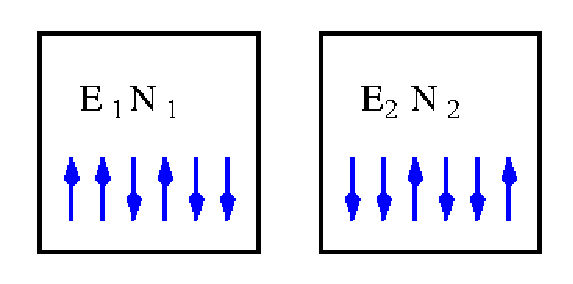
\includegraphics[width=0.7\textwidth]{figs/week02_entropy-separate.pdf}
\end{center}

In the figure above, we can take system $\Om_1$ to have $M_1$ micro-states with probabilities $p_i$ while system $\Om_2$ has $M_2$ micro-states with probabilities $q_k$.
(As discussed above, $M_S$ is a function of $E_S$ and $N_S$ for $S = 1$, $2$.)
Then, even without assuming thermodynamic equilibrium, the entropies of the two systems are
\begin{align*}
  S_1 & = - \sum_{i = 1}^{M_1} p_i \log p_i &
  S_2 & = - \sum_{k = 1}^{M_2} q_k \log q_k.
\end{align*}

\begin{center}
  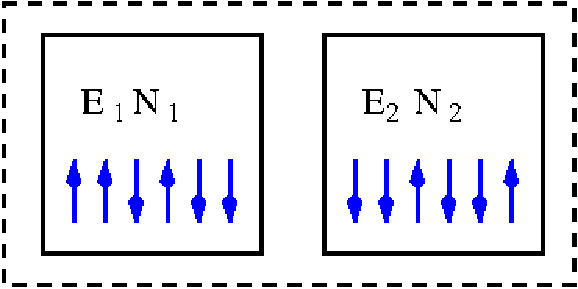
\includegraphics[width=0.7\textwidth]{figs/week02_entropy-combo.pdf}
\end{center}

Now we keep these two (sub)systems isolated from each other, but consider them as a combined system $\Om_{1+2}$, as illustrated above.
In order to compute the entropy $S_{1+2}$, we first need to figure out how many micro-states the combined system could possibly adopt ($M_{1+2}$), and then determine the corresponding probability for each micro-state.
Both steps are simplified by the systems being isolated from each other, so that they are statistically independent.
Specifically, with subsystem $\Om_1$ in a fixed micro-state $\om_i^{(1)}$, subsystem $\Om_2$ could independently inhabit any of its $M_2$ micro-states.
What is the resulting $M_{1+2}$ in terms of $M_1$ and $M_2$?
\begin{mdframed}
  $M_{1+2} = $ \\[50 pt]
\end{mdframed}
Similarly, statistical independence means that the combined probability of subsystem $\Om_1$ adopting micro-state $\om_i^{(1)}$ while subsystem $\Om_2$ adopts $\om_k^{(2)}$ is the product of the individual probabilities, $p_i q_k$.
We can check that this is a well-defined probability, with
\begin{equation*}
  \sum_{M_{1+2}} p_i q_k = \sum_{i = 1}^{M_1} \sum_{k = 1}^{M_2} p_i q_k = \left[\sum_{i = 1}^{M_1} p_i\right]\cdot \left[\sum_{k = 1}^{M_2} q_k\right] = 1\cdot 1 = 1.
\end{equation*}
Inserting the probability $p_i q_k$ into \eq{eq:entropy}, and recalling $\log(a\cdot b) = \log a + \log b$, what is the combined entropy $S_{1+2}$ of these two independent subsystems?
\begin{mdframed}
  $S_{1+2} = $ \\[100 pt]
\end{mdframed}
You should find that the entropies of the two isolated subsystems add up to form the total, which is also the case for the energies and particle numbers,
\begin{align*}
  E_{1+2} & = E_1 + E_2 &
  N_{1+2} & = N_1 + N_2 &
  S_{1+2} & = S_1 + S_2
\end{align*}

\begin{shaded}
  \textbf{Extensive} quantities are \href{https://goldbook.iupac.org/terms/view/E02281}{defined} to be those that add up across independent subsystems.
  Examples include the energy, particle number and entropy as shown above.
  This can be contrasted with \textbf{intensive} quantities, which are \href{https://goldbook.iupac.org/terms/view/I03074}{defined} to be independent of the extent of the system (and hence the same for subsystems as for the combined system).
  We will see an example of this next week. % External magnetic field strength $H$ is control parameter rather than system property...
  It is possible for quantities to be neither extensive nor intensive.
\end{shaded}

Finally, if we were to assume that each subsystem is (independently) in thermodynamic equilibrium, with finite $M_1$ and $M_2$,
\begin{align*}
  p_i & = \frac{1}{M_1} & q_k & = \frac{1}{M_2} \\
  S_1 & = \log M_1      & S_2 & = \log M_2.
\end{align*}
then we would find as a consequence that their combination is also in thermodynamic equilibrium, since
\begin{equation*}
  p_i q_k = \frac{1}{M_1 M_2} = \frac{1}{M_{1+2}}
\end{equation*}
is the same for every combined micro-state.
% ------------------------------------------------------------------



% ------------------------------------------------------------------
\subsubsection{Second law of thermodynamics}
Let's continue considering the two spin (sub)systems discussed above, with one significant change: We suppose the two subsystems are now able to exchange energy (but not particles) with each other.
We'll say they are in \textit{thermal contact} with each other, rather than being fully isolated.
This is illustrated by the figure below:
\begin{center}
  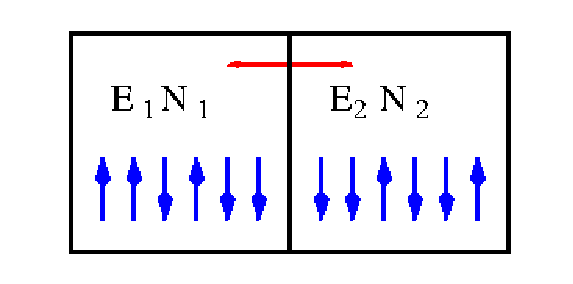
\includegraphics[width=0.7\textwidth]{figs/week02_entropy-exchange.pdf}
\end{center}
The total energy $E = E_1 + E_2$ remains conserved, so the overall system \Om is still governed by the micro-canonical ensemble.
However, the individual energies $E_1$ and $E_2$ can now change as time passes, meaning that \textit{each subsystem is no longer micro-canonical}.

The overall \Om is \textit{not} the same as the combined $\Om_{1+2}$ considered above.
We need to reconsider the total number of micro-states $M$ that \Om could adopt, which is much more difficult than before because we can no longer apply statistical independence.
Our main remaining tool is the conservation of the total energy $E$.

Considering a micro-state in which the $N_1$ spins contribute energy $e_1$ to the total, we know that the $N_2$ spins must contribute the remaining $e_2 = E - e_1$.
Our work above implies there are $M_{e_1} = M_{e_1}^{(1)} M_{E - e_1}^{(2)}$ micro-states providing this particular distribution of energies, where $M_{e_1}^{(1)}$ is the number of micro-states of the formerly isolated subsystem $\Om_1$ with energy $e_1$, and $M_{E - e_1}^{(2)}$ similarly corresponds to $\Om_2$ with energy $E - e_1$.
We also know that it's possible to have $e_1 = E_1$, since that's the initial energy of $\Om_1$ before it was brought into thermal contact with $\Om_2$.
When $e_1 = E_1$, we have $M_{e_1} = M_1 M_2$, covering all the micro-states of the combined system when the two subsystems were isolated.
\textit{In addition}, we also have to count any other microstates for which $e_1 \ne E_1$:
\begin{equation*}
  M = \sum_{e_1} M_{e_1}^{(1)} M_{E - e_1}^{(2)} = M_1 M_2 + \sum_{e_1 \ne E_1} M_{e_1}^{(1)} M_{E - e_1}^{(2)} \geq M_1 M_2.
\end{equation*}
(It could be that $e_1 = E_1$ is the only possibility.)
This is all we can say without specifying more details of a particular example, but it allows us to obtain a famous result for the total entropy $S$ of \Om \textit{in thermodynamic equilibrium}:
\begin{mdframed}
  $S = \log M \geq $ \\[100 pt]
\end{mdframed}

\begin{shaded}
  You have now derived a form of the \textbf{second law of thermodynamics},
  \begin{equation*}
    S \geq S_{1 + 2} = S_1 + S_2.
  \end{equation*}
  In words, whenever isolated (sub)systems in thermodynamic equilibrium are brought into thermal contact with each other and allowed to exchange energy, the total entropy of the overall system can never decrease.
\end{shaded}

This has many far-reaching consequences, the first of which is a more general definition of thermodynamic equilibrium that (unlike \eq{eq:micro_equil}) will also apply when we consider statistical ensembles other than the micro-canonical ensemble.
For simplicity we assume that any system under consideration has a finite number of micro-states, which means that its entropy is bounded from above.
To motivate the definition below, note that the overall system \Om may have undergone an equilibration process to reach its thermodynamic equilibrium after its two (independently equilibrated) subsystems were brought into thermal contact---and in this process the entropy was non-decreasing.

\begin{shaded}
  A system is defined to be in \textbf{thermodynamic equilibrium} if its entropy is maximal.
\end{shaded}

We can \textit{derive} \eq{eq:micro_equil} from this definition.
All we need to do is maximize the entropy $S = - \sum_i p_i \log p_i$ subject (for the micro-canonical ensemble) to the three constraints of conserved energy, conserved particle number, and well-defined probabilities $\sum_i p_i = 1$.
Only the last will turn out to matter, and can be incorporated into the maximization through the method of \textbf{Lagrange multipliers}.
In case you are not familiar with this method, it involves maximizing the modified entropy
\begin{equation*}
  \Sbar = S + \la\left(\sum_{i = 1}^M p_i - 1\right) = - \sum_{i = 1}^M p_i \log p_i + \la\left(\sum_{i = 1}^M p_i - 1\right),
\end{equation*}
where the parameter \la is called the `multiplier'.
In short, this procedure is valid because $\displaystyle \pderiv{\Sbar}{\la} = 0$, so that any extremum of \Sbar corresponds to an extremum of $S$ when the multiplier is set to $\la = 0$.
Recalling $\displaystyle \pderiv{}{x_k} \sum_i f(x_i) = \pderiv{f(x_k)}{x_k}$, what is the probability $p_k$ that maximizes $\Sbar$?
\begin{mdframed}
  $\displaystyle 0 = \pderiv{\Sbar}{p_k} = $ \\[100 pt]
\end{mdframed}
You should find that $p_k$ is some constant that depends on $\la$.
We don't care about $\la$; so long as we know $p_k$ is constant, then $p_k = \frac{1}{M}$ to satisfy $\sum_k p_k = 1$.
As advertised, we recover \eq{eq:micro_equil} from our new definition of thermodynamic equilibrium based on the second law.
% ------------------------------------------------------------------



% ------------------------------------------------------------------
\subsection{Temperature}
In the micro-canonical ensemble, the conserved internal energy and particle number are fundamental, while the temperature (like the entropy) is a derived quantity.
As discussed below \eq{eq:entropy}, in thermodynamic equilibrium such derived quantities are functions of the conserved $\left\{E, N\right\}$.
In this section we will state the definition of temperature for the micro-canonical ensemble and apply this to a spin system.
In the next section we will check that our definition reproduces our expectations from everyday experiences.

\begin{shaded}
  In thermodynamic equilibrium, the \textbf{temperature} in the micro-canonical ensemble is defined by
  \begin{equation}
    \label{eq:temperature}
    \frac{1}{T} = \left. \pderiv{S}{E}\right|_N.
  \end{equation}
  In words, the (inverse) temperature is set by the dependence of the entropy on the internal energy for a fixed number of degrees of freedom.
\end{shaded}

Since this definition is not terribly intuitive, we will again gain insight by working through the \textbf{example} of $N$ spins in a line, in an external magnetic field of strength $H$.
We saw above that $E = H(n_+ - n_-)$ for $n_+$ and $n_- = N - n_+$ spins respectively aligned anti-parallel and parallel to the magnetic field.
Each (conserved) value of $E$ defines a \textit{different} micro-canonical system, which we can expect to have a different number of micro-states $M(E)$, different entropy $S(E)$ and different temperature $T(E)$.
We will compute the functional forms of each of these three quantities, starting with $M(E)$.

Even though the total energy $E$ remains fixed as time passes, individual spins can `flip' between pointing parallel or anti-parallel to the magnetic field.
Such spin flips simply have to come in pairs so that the overall $n_{\pm}$ both remain the same.
As illustration, what are the spin configurations that produce the minimal energy $E_{\text{min}} \equiv E_0$ and the next-to-minimal $E_1$?
What are $E_0$ and $E_1$ in terms of $\left\{N, H\right\}$, and how many distinct micro-states are there for each of $E_0$ and $E_1$?
\begin{mdframed}
  \ \\[100 pt]
\end{mdframed}
Your results should generalize to
\begin{equation}
  \label{eq:spin_states}
  M(E_{n_+}) = \binom{N}{n_+} = \frac{N!}{n_+! \; (N - n_+)!}.
\end{equation}

To take the derivative in \eq{eq:temperature}, we need to express $n_+$ in terms of $\left\{E, N\right\}$.
It will also be convenient to avoid the factorial operation, which is inconvenient to differentiate.
For $N \gg 1$, we can accomplish both these goals by interpreting the spin system as a random walk (in the abstract `line' of its possible energies $E$) and applying the central limit theorem: \\[-24 pt]
\begin{itemize}
  \item Each spin adds to $x \equiv \frac{E}{H} = 2n_+ - N$ a `step' of fixed `length' $\pm 1$.
        Our task therefore coincides with the special case we considered in \secref{sec:diffusion}.
  \item We don't impose any preference for positive vs.\ negative energies, meaning $p = q = \frac{1}{2}$ in the language of \secref{sec:diffusion}.
  \item With $p = q = \frac{1}{2}$, every one of the $2^N$ possible configurations of $N$ spins is equally probable.
        Therefore the probability $P_{n_+}$ that our overall `walk' ends up producing a configuration with $n_+ = \frac{1}{2}\left(x + N\right)$ is simply the fraction of those $2^N$ configurations with this $n_+$, in which we can recognize \eq{eq:spin_states}:
        \begin{equation*}
          P_{n_+} = \frac{1}{2^N} \binom{N}{n_+} = \frac{M(E_{n_+})}{2^N} \qquad \implies \qquad M(E_{n_+}) = 2^N P_{n_+}.
        \end{equation*}
  \item To estimate $P_{n_+}$ for $N \gg 1$, we apply the central limit theorem just as in \secref{sec:RW_CLT}.
        In particular, we can re-use our computation that $\mu = 2p - 1 = 0$ and $\si^2 = 4pq = 1$, finding
        \begin{equation*}
          p(x) = \frac{1}{\sqrt{2\pi N}}\exp\left[-\frac{x^2}{2N}\right] = \frac{1}{\sqrt{2\pi N}}\exp\left[-\frac{E^2}{2NH^2}\right]
        \end{equation*}
        for the probability \textit{distribution} from which we want to extract $P_{n_+}$.
  \item We saw in \secref{sec:CLT} that $P_{\text{const}}(n_+) = p(2n_+ - N) \De n_+$ is a good approximation, and $\De n_+ = 1$.
        Therefore we find
        \begin{equation}
          \label{eq:CLT_states}
          M(E) \approx 2^N p(2n_+ - N) \approx \frac{2^N}{\sqrt{2\pi N}}\exp\left[-\frac{E^2}{2NH^2}\right].
        \end{equation}
\end{itemize}
What is the derivative of the log of \eq{eq:CLT_states} with $N$ fixed?
\begin{mdframed}
  $\displaystyle \left.\pderiv{}{E} \log M\right|_N = $ \\[100 pt]
\end{mdframed}

You should find the temperature
\begin{align}
  T & \approx -\frac{NH^2}{E} &
  N & \gg 1,
\end{align}
which in several ways does \textit{not} seem to match our expectations from everyday experiences: This $T$ diverges as $E \to 0$ for $n_+ \approx n_-$, and it is negative whenever $E > 0$ (corresponding to $n_+ > n_-$).\footnote{You can check that $T < 0$ whenever the number of micro-states decreases for larger internal energies, $\pderiv{M}{E} < 0$.  In so-called `natural' systems, larger energies `open up' more possible micro-states, producing $\pderiv{M}{E} > 0$ and a positive temperature.}
When $H = 0$, we also have $E = 0$ and $T$ is ill-defined.
Restricting our attention to $H > 0$, with $n_+ < n_-$ producing a positive temperature, we also see that this temperature cannot vanish.
It is minimized by the most-negative energy you found above, $T_{\text{min}} = H > 0$ for $E_{\text{min}} = -NH$.
The non-zero minimum temperature is specific to spin systems, while some of the other oddities result from the micro-canonical approach more generally.
This will motivate turning to the canonical ensemble next week, but first we can check that at least some aspects of the temperature defined in \eq{eq:temperature} do match with our everyday expectations.
% ------------------------------------------------------------------



% ------------------------------------------------------------------
\subsection{Heat exchange}
When a high-temperature system $A$ is brought into thermal contact with a low-temperature system $B$, we expect from everyday experiences that $A$ will cool down heating up $B$.
We will now check that the micro-canonical definition of temperature in \eq{eq:temperature} predicts this behaviour.

\TODO{Being written...}
% ------------------------------------------------------------------
